At the backbone of all classical protocols described in Section \ref{section:protocols}, it lies the need to generate random uniform distributions of either qubit states, Bloch vectors or shared randomness in $\mathbb{R^3}$. In Figure \ref{fig:results_random_states}, we can see that applying random unitary transformations to zero qubit states leads to uniformly distributed random qubit pure states, which can later be transformed into random Bloch vectors or normalized random vectors in $\mathbb{R^3}$ as needed.
\begin{figure}[h]
\centering
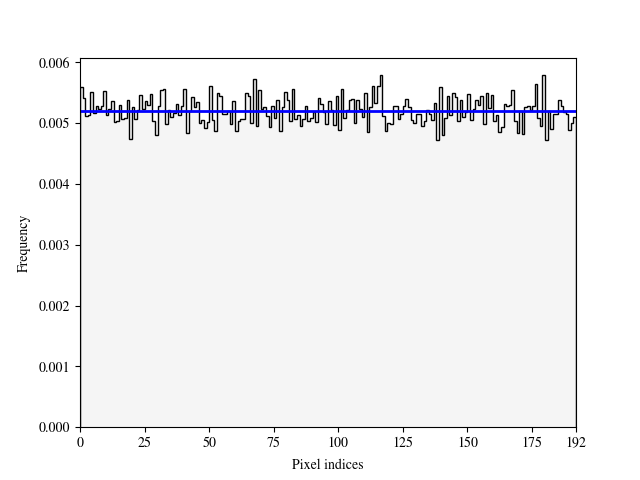
\includegraphics[width=\textwidth]{images/random_bloch_healpix.png}
\caption{In this figure, we see how the frequency distribution of $N=10^4$ random qubit states generated with \cite{software2023} follows a random uniform distribution of state vectors along the Bloch sphere (blue solid line). The frequencies are binned by HEALPix indices corresponding to an orthographic partition of the Bloch sphere with resolution $\mathit{NSIDE}=4$.}
\label{fig:results_random_states}
\end{figure}

\textit{To be included:}

\textit{Random states verification}

\textit{Convergence plots, classical vs. quantum vs. theoretical probabilities}

\textit{Kullback-Leibler divergence plots}

\textit{Quantum Simulator vs. NISQ Computer benchmarking}

\textit{Bell scenario joint probabilities convergence}

\textit{CHSH inequality}